\section[Introdução]{Introdução}
Desenvolvido para o \ac{mprs}, o projeto Vincula visa solucionar uma necessidade crítica do \ac{nimp}: a ausência de uma ferramenta integrada para cruzamento de dados recebidos em investigações, como os de quebras de sigilo bancário e telefônico.

O processo atual é manual e fragmentado, o que dificulta a identificação de relações complexas. Para resolver esse problema, nosso objetivo é desenvolver uma plataforma web que permita aos analistas e promotores visualizar os vínculos entre as informações de forma gráfica e intuitiva, além de gerar relatórios.

O projeto, que está sendo desenvolvido durante o segundo semestre de 2025, conta com a orientação do Prof. Dilnei Venturini e a colaboração direta dos stakeholders Césio Luiz Velleda Lázaro da Silva e Luciano Ratai Menna Barreto. A \autoref{fig:time-vincula} mostra o time reunido com o professor e os stakeholders.

\begin{figure}[H]
    \centering
    \small
    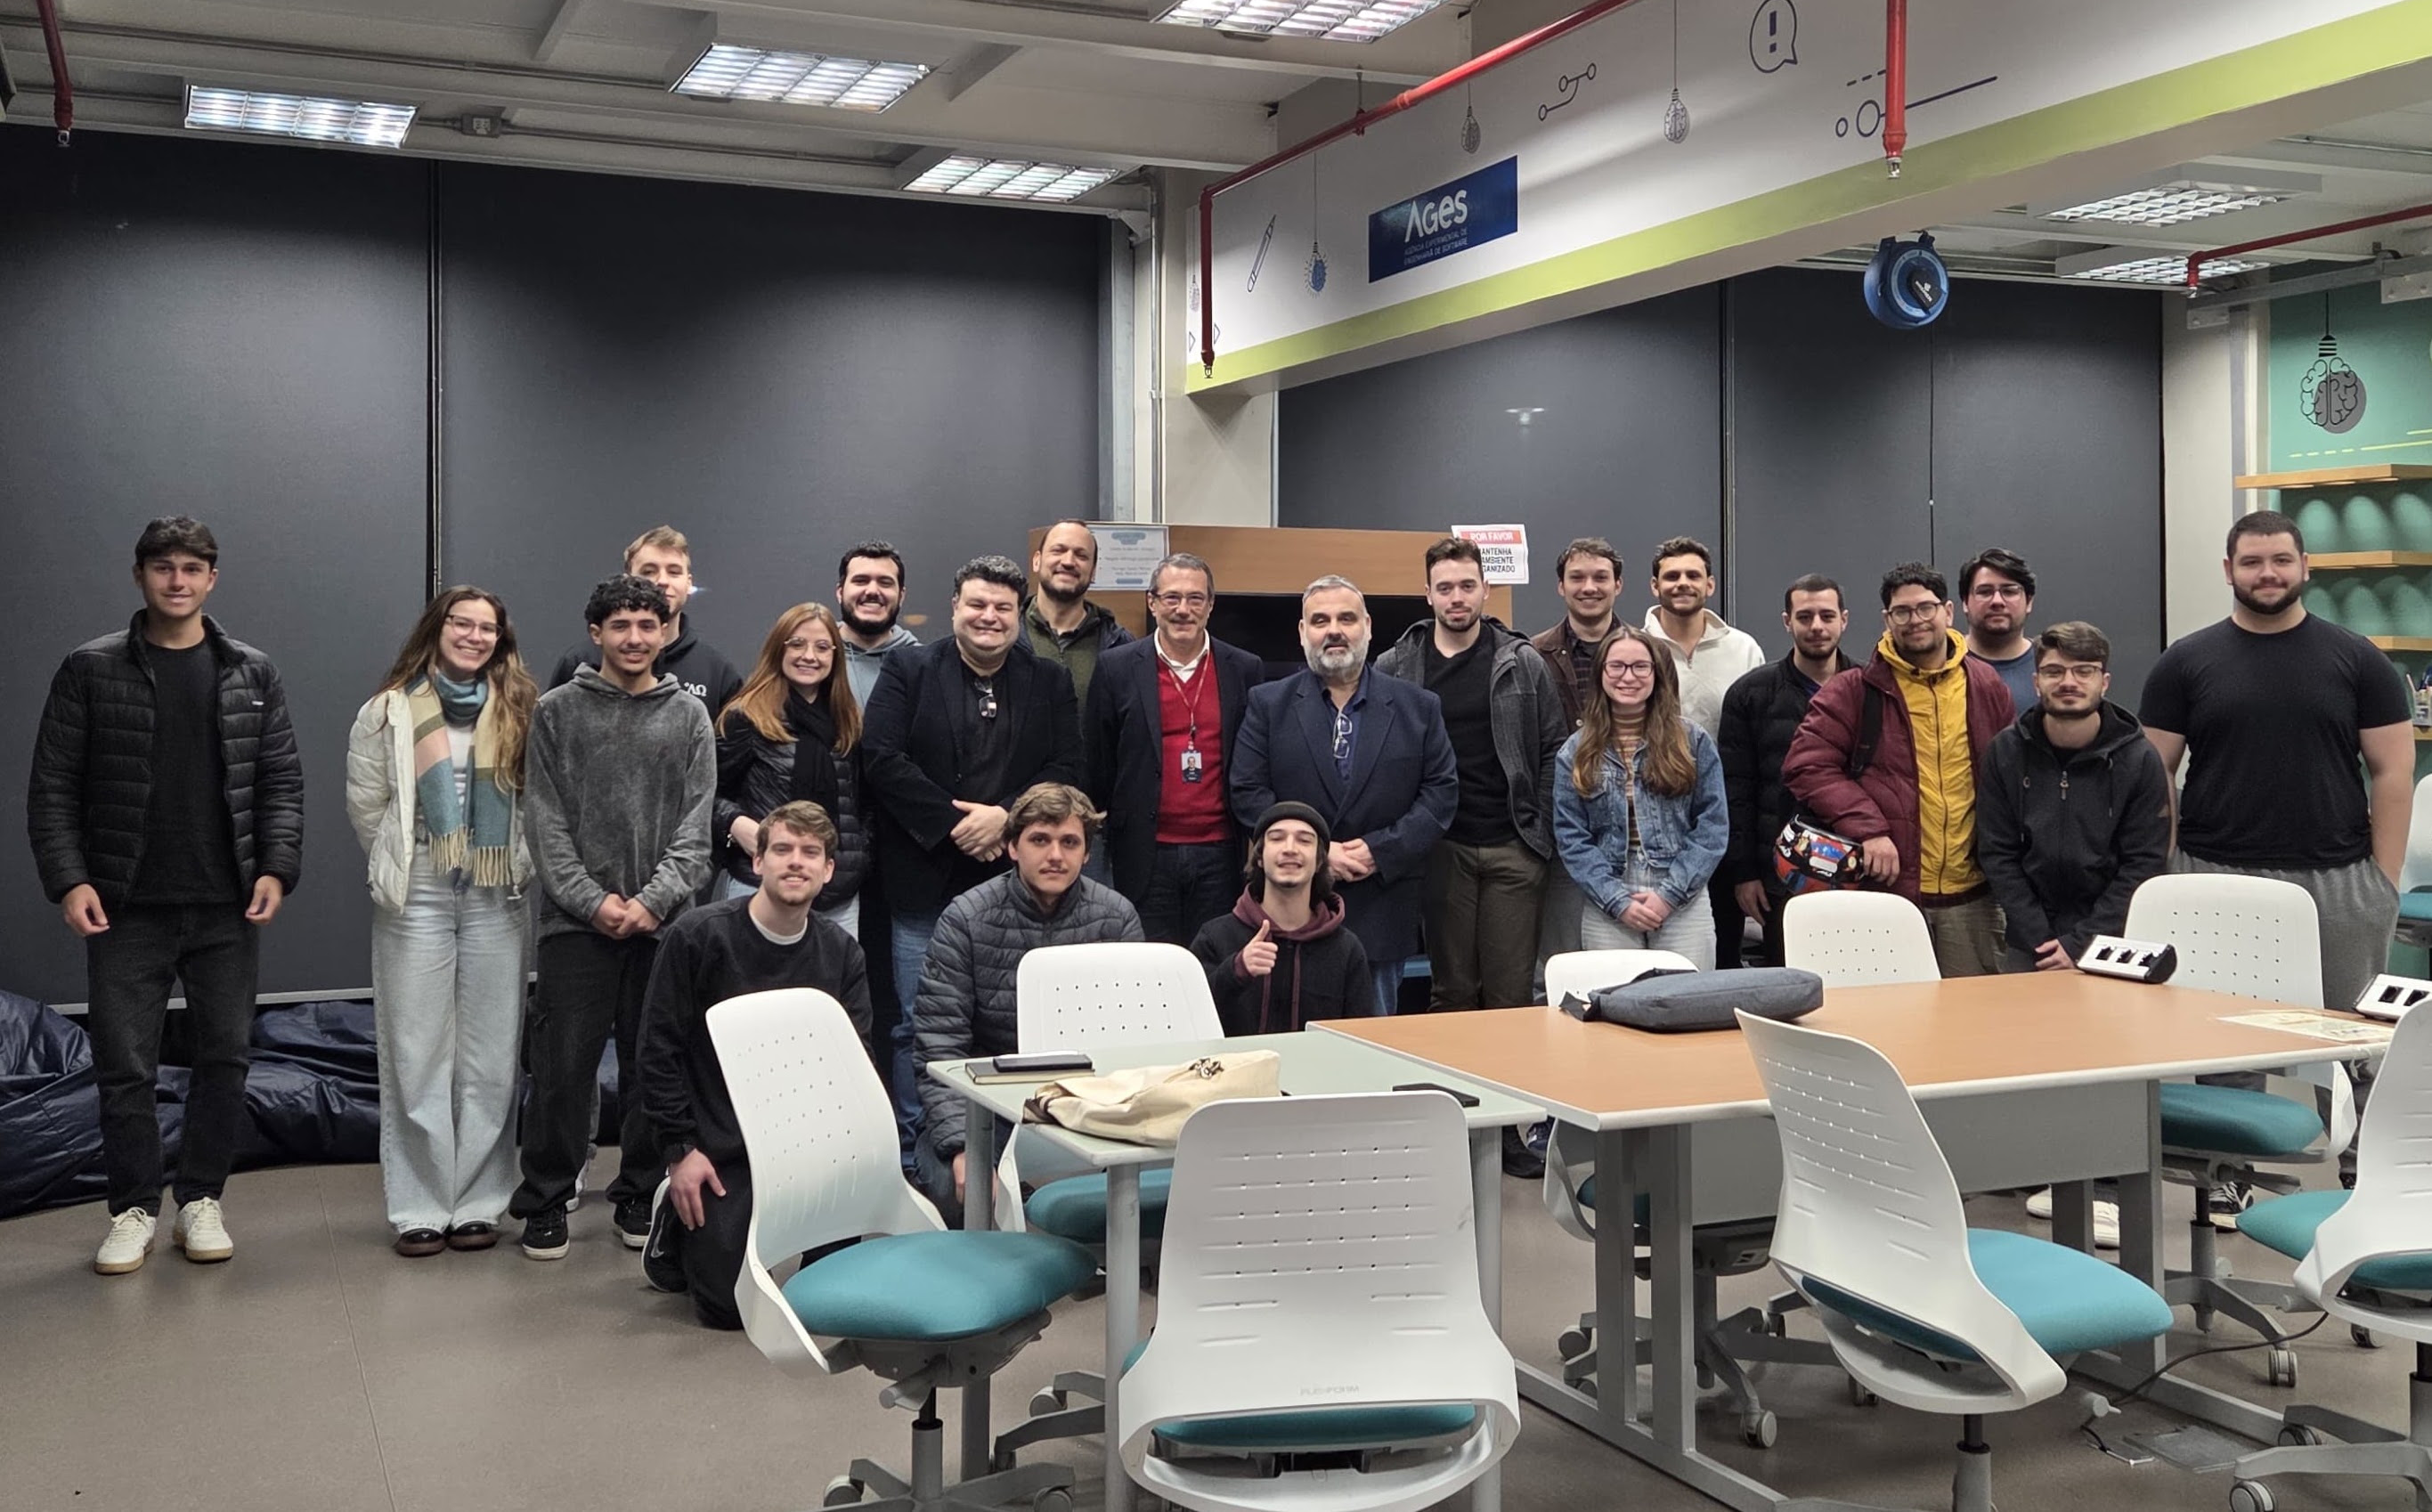
\includegraphics[width=1\linewidth]{conteudo//2 - ages I//conteudo//figures//foto-time.jpg}
    \caption{Time Vincula}
    Fonte: Adaptado de \textcites{wiki-vincula}
    \label{fig:time-vincula}
\end{figure}